% !TeX root = documentation.tex
% !TeX spellcheck = de_DE

\section{Analyse der Gleichungen}
Die Gleichungen, welche das Lorenz-Modell beschreiben, enthalten viele physikalische Eigenschaften wie die Dichte, Geschwindigkeit und Temperatur der Atmosphäre und stellen diese physikalischen Werte formalisiert dar. Lorenz wollte aus den bereits existierenden Gleichungen der Hydrodynamik ein Modell zur Wetterprognose erstellen. Basierend auf vorgehende Werke von Saltzman startete Lorenz mit den hyrodynamischen Gleichungen und verfolgte ein systematisches Näherungsvorgehen, womit er auf die folgenden drei Gleichungen stoss:

\begin{centerFigure}
	\begin{align}
	\dot{x} &= \sigma(x - y)\\
	\dot{y} &= x(\rho - z) - y\\
	\dot{z} &= xy - \beta z
	\end{align}
\end{centerFigure}

Die X-Achse entspricht dabei der hydrodynamischen, räumlichen Durchschnittsgeschwindigkeit, also wie wir verstanden haben, durschnittliche Windgeschwindigkeit. 
Die Y-Achse repräsentiert die Temperatur und die Z-Achse der Temperaturgradient. Also wie schnell sich die Temperatur verändert. 

Wie aus den obigen Gleichungen ersichtlich ist, sind drei Parameter vorhanden. Alle sind immer positiv.

\subsubsection{1. Parameter: $\sigma$}
$\sigma$ entspricht der dimensionslosen Prandtl Nummer. Diese ist das Verhältnis von \textit{Viskosit"at} und der \textit{Temperaturleitfähigkeit}. Da beide Eigenschaften die Einheit $\frac{m^2}{s}$ haben, resultiert daraus eine dimensionslose Zahl.

\subsubsection{2. Parameter: $\rho$}
Auch das $\rho$ wurde nach einem Mathematiker benannt. Der Name für diesen Parameter ist Rayleigh Nummer. Es entspricht dem Verhältnis von \textit{W"armeausdehnung} und der \textit{Viskosit"at}.

\subsubsection{3. Parameter: $\beta$}
Der dritte Parameter des Lorenz-Modells ist das $\beta$. Es entspricht der W"armeausdehnung. Dabei handelt es sich um die Ver"anderung der geometrischen Gr"ossen eines K"orpers, die sich mit erh"ohter Temperatur vergr"ossern. Dehnt sich ein K"orper aufgrund der Temperatur"anderung aus, so ver"andert sich auch stets die Dichte. Bei fluiden Materialien hat dies Auswirkungen auf den Druck. 

\subsection{Implementation}

\paragraph{Lorenz-System}
Differenzialgleichungslöser in Javascript implementieren ist sehr ineffizient und auch gar nicht nötig. Wir haben uns für einen anderen Weg entschieden. Das Ergebnis einer Differenzialgleichung ist die Steigung an einem Punkt t. Diese Steigung können wir in eine lineare Gleichung einsetzen und daraus den absoluten Punkt berechnen.

Der \textit{Y-Achsenabschnitt} wird mit dem Ergebnis der vorherigen Rechnungsschritt belegt, da der Differenzalterm den Abstand vom Wert \textit{vorher} berechnet.  

\begin{align}
\label{LGResult}
y(t + 1) &= \frac{\delta LG}{\delta t} * \Delta + y(t) & LG = Lorenzgleichung
\end{align}

Dieses Verfahren kann auf alle Koordinaten des Lorenz-Systems angewendet werden.

Eingefügt in die Gleichung \eqref{LGResult} ergibt sich folgendes System:

\begin{centerFigure}
\begin{align}
x(t + 1) &= \frac{\delta \sigma(x - y)}{\delta t} * \Delta + x(t)\\
y(t + 1) &= \frac{\delta x(\rho - z) - y}{\delta t} * \Delta + y(t)\\
z(t + 1) &= \frac{\delta xy - \beta z}{\delta t} * \Delta + z(t)
\end{align}
\end{centerFigure}
Das angewendete Verfahren nennt sich \textit{Eulerisches-} oder \textit{Einschritt-Verfahren}. Durch das, dass wir einen numerischen Ansatz mit dem Euler Verfahren gew"ahlt haben, resultiert eine Ann"aherung des Lorenz-Attraktors. Da solche Abweichungen von der tats"achlichen L"osung existieren, ist zu erwarten, dass diese Abweichungen gross genug sind, um zum chaotischen Verhalten beizutragen. Es g"abe auch genauere Verfahren f"ur das numerische L"osen der Gleichungen wie das \textit{Quadratische Verfahren} oder das \textit{Runge-Kutta Verfahren}. Da aber auch bei diesen Verfahren keine absolute Genauigkeit erreicht wird, blieben wir bei der Eulerischen Ann"aherung. \\

Das oben erw"ahnte Gleichungssystem haben wir im Javascript-Code verwendet, um die Resultate des Lorenzsystems auszurechnen. In Javascript haben wir die Punkte in einem Array(\texttt{Tuple3}) gespeichert.

\begin{centerFigure}[Formeln im Code]
\begin{lstlisting}
x = arr[i].x + ((sigma * y) - (sigma * x)) * delta;
y = arr[i].y + ((-x * z) + (rho * x) - y) * delta;
z = arr[i].z + ((x * y) - (beta * z)) * delta;
\end{lstlisting}
\end{centerFigure}

Die $ x, y $ Variablen in der 1. Gleichung ist noch mit dem Wert des vorherigen Durchgangs besetzt und deshalb eine Annäherung um den echten Wert. Das gleiche gilt für alle Werte, die vor der Ausführung noch nicht gesetzt sind. Beim ersten Durchgang wird 0.1 als Startwert angenommen. Die folgenden Variablen wurden für den Code verwendet und definiert:

\begin{centerFigure}[Variablen des Codes]
	\begin{tabular}{| c | c |}
		\hline
		delta $ (\Delta) $ & 0.1 \\\hline
		sigma $ (\sigma) $ & \multirow{3}{*}{Argumente}\\
		rho $(\rho) $ & \\
		beta $ (\beta) $ & \\\hline
		x & \multirow{3}{*}{berechnet}\\
		y & \\
		z & \\\hline
	\end{tabular}
\end{centerFigure}

\paragraph{Visualisierung}
Die Werte des Lorenz-Systems, welche der Algorithmus im letzten Paragraph berechnet hat, stellen Ortsvektoren in einem drei dimensionalen Raum dar. An jedem Punkt des Lorenz-Systems stellt der Visualisierungsalgorithmus eine \textit{Sphere} dar. Es werden in unserer Darstellung 2500 Werte berechnet und angezeigt.

\begin{centerFigure}[Visualisierung des Lorenz Attraktors]
	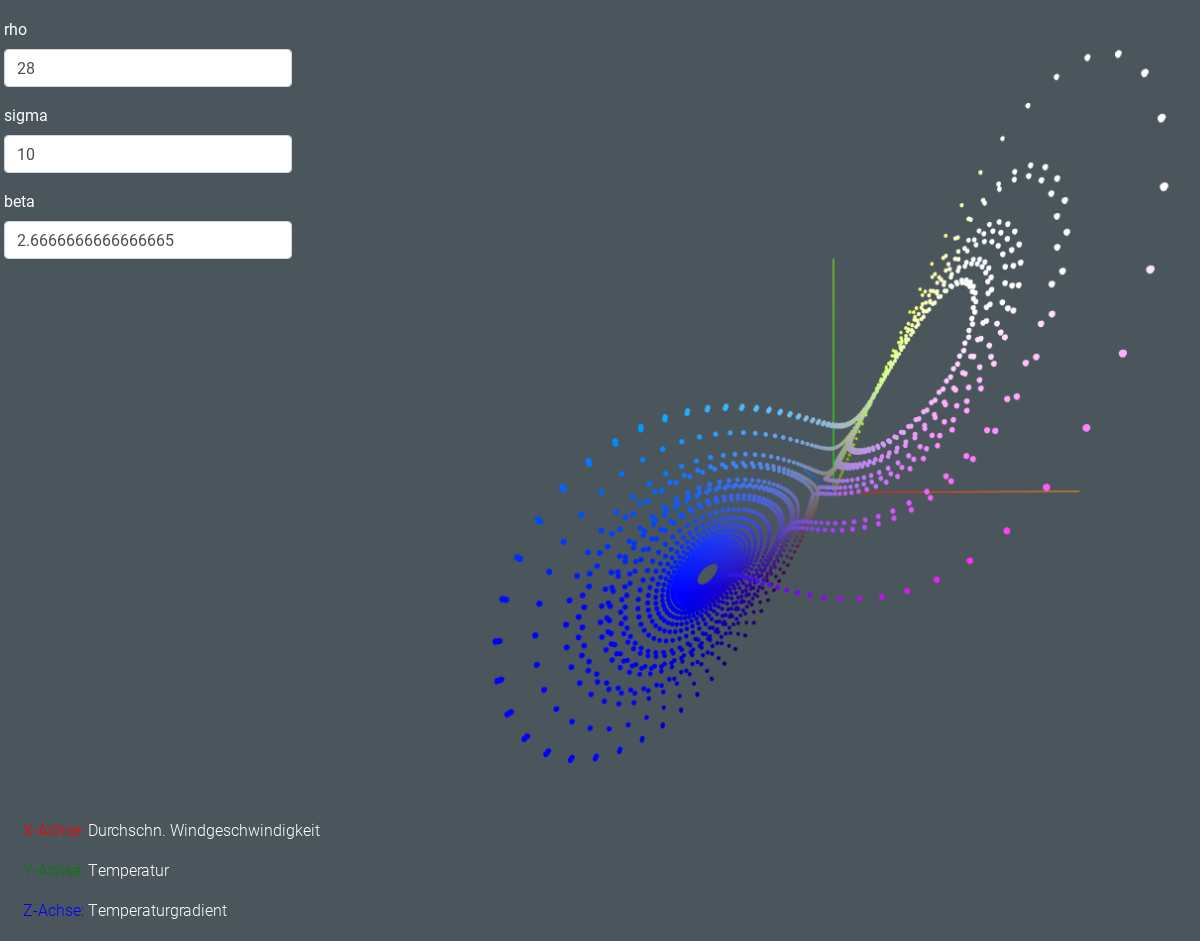
\includegraphics[height=5cm]{lorenz/assets/implementation/Visualisierung}
\end{centerFigure}

